\subsection{Reduced centipede game}
\paragraph{Answers}

\subsubsection{Use backward induction to predict the (rational) outcome of this game. Does it make sense to you?}


\begin{figure}[ht]
    \centering
    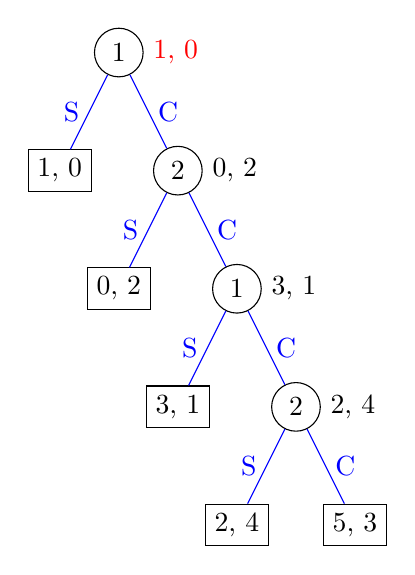
\begin{tikzpicture}
        \node[circle, black,draw, label={[red]right: 1, 0}] {1}
            child {node[draw] {1, 0} edge from parent [left, blue] node {S}}
            child {node[circle, black, draw, label={right: 0, 2}] {2}
            child {node [draw, black] {0, 2}
            edge from parent [left, blue] node {S}}
            child {node [circle, black,draw, label={right: 3, 1}]{1}
            child {node [draw, black] {3, 1}
            edge from parent [left, blue] node {S}}
            child {node [circle, black,draw, label={right: 2, 4}] {2}
            child {node [draw, black] {2, 4}
            edge from parent [left, blue] node {S}}
            child {node [draw, black] {5, 3}
            edge from parent [right, blue] node {C}}
            edge from parent [right, blue] node {C}}
            edge from parent [right, blue] node {C}} 
            edge from parent [blue] node [right, blue] {C}};
    \end{tikzpicture}
\end{figure}
The rational outcome of this game is 1, 0. Given that the utility of both players increases along
the game tree, both players could get better pay-offs. If both players would be altruistic instead
of maximizing their own outcome, they would both go down the tree and would both receive better 
pay-offs.

\subsubsection{Write the normal form for this game and find all Nash equilibria in pure strategies (PNEs).}


\begin{table}[h!]
  \centering
  \begin{tabular}{|l|l|l|l|l|}
    \hline
           &   SS          &  SC           &  CS  &   CC \\ \hline
       SS  & \textbf{1, 0} & \textbf{1, 0} & 1, 0 & 1, 0 \\ \hline
       SC  & \textbf{1, 0} & \textbf{1, 0} & 1, 0 & 1, 0 \\ \hline
       CS  & 0, 2          & 0, 2          & 3, 1 & 3, 1 \\ \hline
       CC  & 0, 2          & 0, 2          & 2, 4 & 5, 3 \\ \hline
  \end{tabular}
  \caption{Normal Form for the Reduced centipede game, with PNEs in bold.}
  \label{your-table-label}
\end{table}



\subsubsection{List all subgames and determine which of these PNEs are also subgame-perfect?}
\begin{figure}[ht]
  \centering
  \begin{subfigure}[b]{0.3\textwidth}
    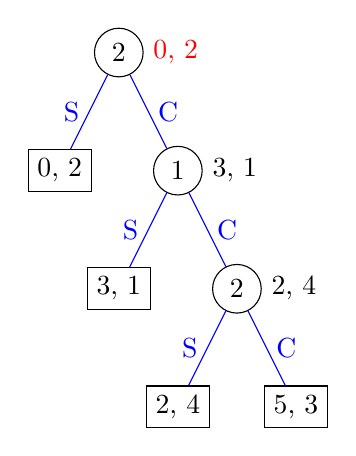
\begin{tikzpicture}
        \node[circle, black, draw, label={[red]right: 0, 2}] {2}
            child {node [draw, black] {0, 2}
            edge from parent [left, blue] node {S}}
            child {node [circle, black,draw, label={right: 3, 1}]{1}
            child {node [draw, black] {3, 1}
            edge from parent [left, blue] node {S}}
            child {node [circle, black,draw, label={right: 2, 4}] {2}
            child {node [draw, black] {2, 4}
            edge from parent [left, blue] node {S}}
            child {node [draw, black] {5, 3}
            edge from parent [right, blue] node {C}}
            edge from parent [right, blue] node {C}}
            edge from parent [right, blue] node {C}};
    \end{tikzpicture}
    \subcaption*{equilibria: (SS, SS), (CS, SC)}
  \end{subfigure}
  \begin{subfigure}[b]{0.3\textwidth}
    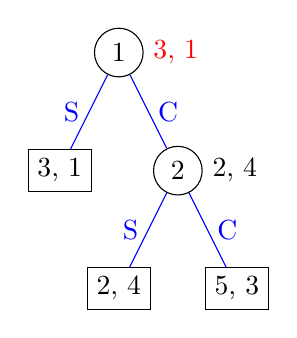
\begin{tikzpicture}
      \node[circle, black,draw, label={[red]right: 3, 1}]{1}
          child {node [draw, black] {3, 1}
          edge from parent [left, blue] node {S}}
          child {node [circle, black,draw, label={right: 2, 4}] {2}
          child {node [draw, black] {2, 4}
          edge from parent [left, blue] node {S}}
          child {node [draw, black] {5, 3}
          edge from parent [right, blue] node {C}}
          edge from parent [right, blue] node {C}};
  \end{tikzpicture}
  \subcaption*{equilibria: (SS, SS), (CS, SS), (SS, CS), (CS, CS) (both players have to play S as seconds choice)}
  \end{subfigure}
  \begin{subfigure}[b]{0.3\textwidth}
    \centering
    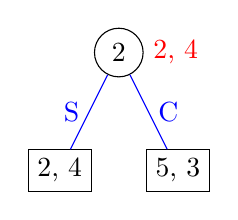
\begin{tikzpicture}
      \node[circle, black,draw, label={[red]right: 2, 4}] {2}
          child {node [draw, black] {2, 4}
          edge from parent [left, blue] node {S}}
          child {node [draw, black] {5, 3}
          edge from parent [right, blue] node {C}};
    \end{tikzpicture}
    \subcaption*{equilibria: (**, *S)}
  \end{subfigure} 
\end{figure}
\newpage
The only equilibrium present in all sub-games and the game itself is (SS, SS).